% Author: Dai Nguyen
% Document type: CV/Resume

\documentclass[letterpage]{article}

%%%%%%%%%%%%%%%%%%%%%%%%%%%%%%%%%%%%%
% DEFINE DEFAULT FONT STYLE
%%%%%%%%%%%%%%%%%%%%%%%%%%%%%%%%%%%%%
\usepackage{fontawesome}
\usepackage[defaultsans]{cantarell}
\usepackage[default,scale=0.95]{carlito}
\usepackage[T1]{fontenc}
\fontsize{10px}{0.45px}\selectfont
\usepackage{lmodern}

%%%%%%%%%%%%%%%%%%%%%%%%%%%%%%%%%%%%%
% DEFINE PAGE LAYOUT & SPACING
%%%%%%%%%%%%%%%%%%%%%%%%%%%%%%%%%%%%%
% For NO HYPHEN
\tolerance=1
\emergencystretch=\maxdimen
\hyphenpenalty=10000
\hbadness=10000
% NO HYPHEN END
\usepackage[top=0.3in, bottom=0.4in, left=0.55in,
right=0.85in]{geometry}
\usepackage{setspace}              % for line spacing
\usepackage{vwcol}                  % unused - columns with different widths
\usepackage{multicol}               % unused - for columns with equal widths
                                       	% currently using minipage to create columns
\usepackage{enumitem}           	% for 'itemize' configuration
% http://ctan.org/pkg/enumitem
% bullet style for items in list:
\renewcommand\labelitemi{\rule[1mm]{0.33mm}{0.33mm}}  

%%%%%%%%%%%%%%%%%%%%%%%%%%%%%%%%%%%%%
% COLOR PACKAGE & PREDEFINED COLORS
%%%%%%%%%%%%%%%%%%%%%%%%%%%%%%%%%%%%%
\usepackage[dvipsnames]{xcolor}
\definecolor{white-smoke}{HTML}{F2F7F8}
\definecolor{arsenic}{HTML}{40424A}
\definecolor{light-sky-blue}{HTML}{87CBFF}
\definecolor{brilliant-azure}{HTML}{3AB0FF}
\definecolor{beaublue}{rgb}{0.74, 0.83, 0.9}
\definecolor{ceil}{rgb}{0.57, 0.63, 0.81}
\pagecolor{white-smoke}
\AtBeginDocument{\color{arsenic}}

%%%%%%%%%%%%%%%%%%%%%%%%%%%%%%%%%%%%%
% OTHER PACKAGES
%%%%%%%%%%%%%%%%%%%%%%%%%%%%%%%%%%%%%
\usepackage{array,multirow,graphicx} 		% for tables
\usepackage{verbatim}                 		% for multi-line comments
\usepackage{graphicx}                  		% for rotating text boxes
\usepackage{tikz}                      		% for drawing shapes & highlights
\usepackage{soul}                      		% for text highlights/underlines
\setul{-0.5ex}{1ex}                    		% set underline dimension
\setuloverlap{3pt}                     		% how much line is sticking out
\setulcolor{ceil}                 			% set undline color for package soul
\usepackage{amssymb,amsmath}
\usepackage{mathabx}                   % for math symbols
\usepackage{ifxetex,ifluatex}
\usepackage{fixltx2e}                  % provides \textsubscript
\ifnum 0\ifxetex 1\fi\ifluatex 1\fi=0  % if pdftex
  \usepackage[T1]{fontenc}
  % Setup & declare Unicode characters
  \usepackage[utf8]{inputenc}
  \DeclareUnicodeCharacter{0160}{\^--}
\else % if luatex or xelatex
  \ifxetex
    \usepackage{mathspec}
  \else
    \usepackage{fontspec}
  \fi
  \defaultfontfeatures{Ligatures=TeX,Scale=MatchLowercase}
\fi
% use upquote if available, for straight quotes in verbatim
% environments
\IfFileExists{upquote.sty}{\usepackage{upquote}}{}
% use microtype if available
\IfFileExists{microtype.sty}{%
\usepackage{microtype}
\UseMicrotypeSet[protrusion]{basicmath}
% ^ disable protrusion for tt fonts
}{}
\usepackage[unicode=true]{hyperref}
\hypersetup{
            pdfborder={0 0 0},
            breaklinks=true}
\urlstyle{same}               % don't use monospace font for urls
\usepackage{graphicx,grffile} % for inserting pictures
\makeatletter
\def\maxwidth{\ifdim\Gin@nat@width>\linewidth\linewidth\else
\Gin@nat@width\fi}
\def\maxheight{\ifdim\Gin@nat@height>\textheight\textheight\else
\Gin@nat@height\fi}
\makeatother
% Scale images if necessary, so that they will not overflow 
% the page margins by default, and it is still possible to
% overwrite the defaults using explicit options in
% \includegraphics[width,height, ...]{}
\setkeys{Gin}{width=\maxwidth,height=\maxheight,keepaspectratio}
\IfFileExists{parskip.sty}{%
\usepackage{parskip}
}{% else
\setlength{\parindent}{0pt}
\setlength{\parskip}{6pt plus 2pt minus 1pt}
}
\setlength{\emergencystretch}{3em}  % prevent overfull lines
\providecommand{\tightlist}{%
  \setlength{\itemsep}{0pt}\setlength{\parskip}{0pt}}
\setcounter{secnumdepth}{0}
% Redefines (sub)paragraphs to behave more like sections
\ifx\paragraph\undefined\else
\let\oldparagraph\paragraph
\renewcommand{\paragraph}[1]{\oldparagraph{#1}\mbox{}}
\fi
\ifx\subparagraph\undefined\else
\let\oldsubparagraph\subparagraph
\renewcommand{\subparagraph}[1]{\oldsubparagraph{#1}\mbox{}}
\fi

\begin{document}
\thispagestyle{empty} % to remove page number
%%%%%%%%%%%%%%%%%%%%%%%%%%%%%%%%%%%%%
% HEADER: NAME & INFOMARTION
%%%%%%%%%%%%%%%%%%%%%%%%%%%%%%%%%%%%%
\begin{minipage}[c]{0.4\linewidth}
  \raggedright
  \textbf{\fontsize{37px}{1px}\selectfont\textsf{DAI}}\\
  \vspace{7px}
  {\fontsize{37px}{1px}\selectfont\textsf{NGUYEN}}
\end{minipage}
\begin{minipage}{0.01\linewidth}
  % INTENTIONALLY LEFT BLANK
\end{minipage}
\:\:\:\:\: % space between minipages
%\begin{minipage}[t]{0.31\linewidth}
%  \raggedleft
%  \vspace*{-30px}
%  Atlanta, GA\enspace\faGlobe\\
%  dai-nguyen.com\enspace\faGlobe\\
%  hire@dai-nguyen.com\enspace\faPaperPlane\\
%  linkedin.dai-nguyen.com\enspace\faLinkedin\\
%  github.dai-nguyen.com\enspace\faGithubAlt\\
%\end{minipage}
%\:\:\:\:\: % space between minipages
%\begin{minipage}[c]{0.2\linewidth}
%  \raggedright
%  \begin{tikzpicture}
%    \fill[ceil] (0,2.2) circle (1.2);
%    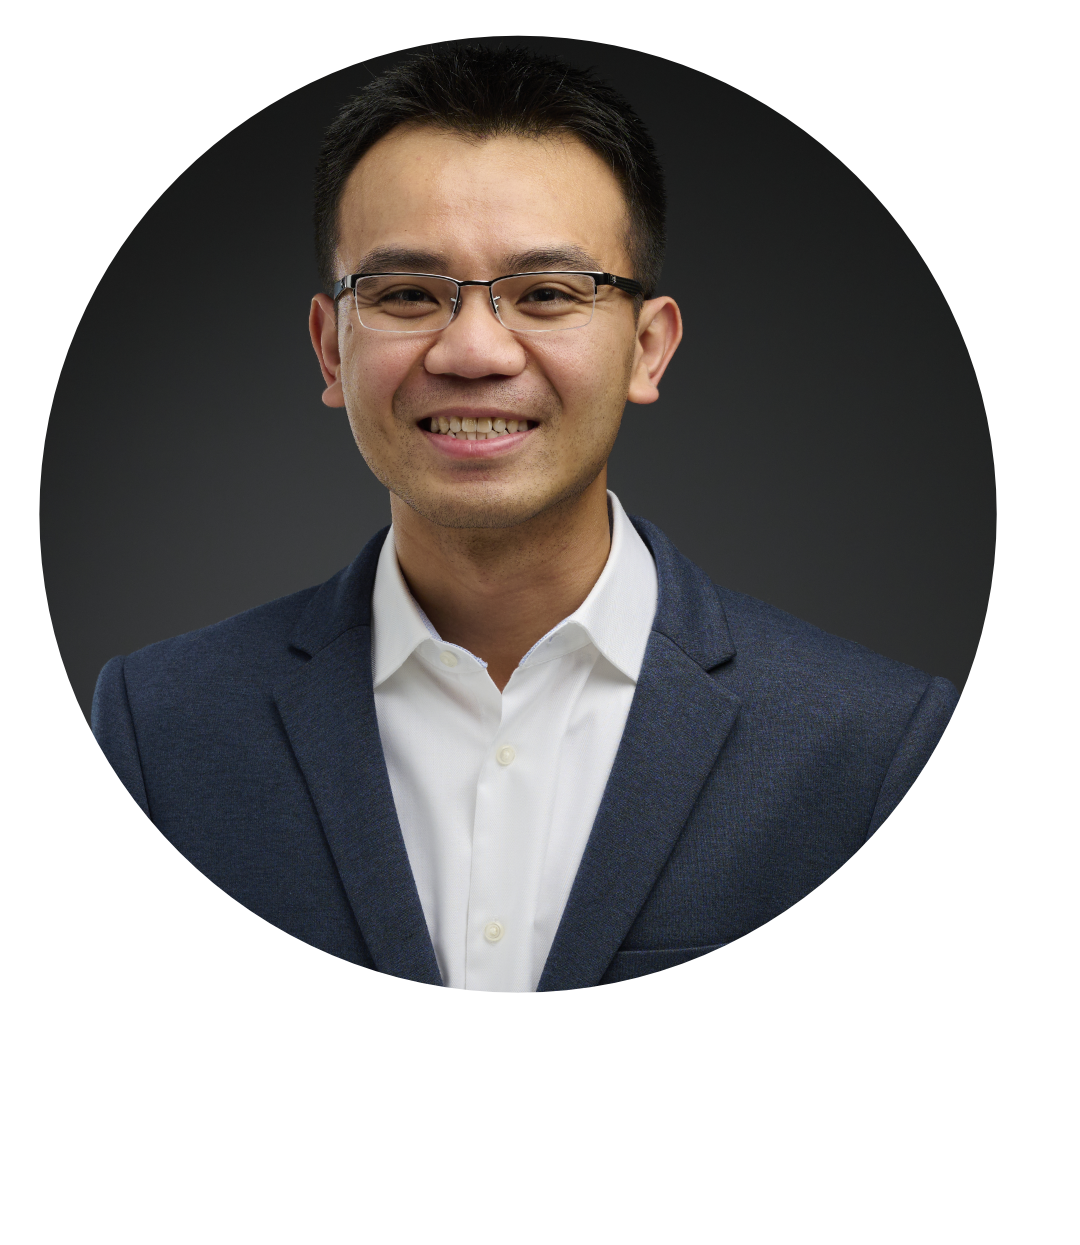
\includegraphics[width=1\linewidth]{assets/images/profile.png}
%  \end{tikzpicture}
%\end{minipage}
\begin{minipage}[t]{0.6\linewidth}
  \raggedleft
  \vspace*{-30px}
  Atlanta, GA, USA\enspace\faGlobe\\
  dai-nguyen.com\enspace\faGlobe\\
  hire@dai-nguyen.com\enspace\faPaperPlane\\
  linkedin.dai-nguyen.com\enspace\faLinkedin\\
  github.dai-nguyen.com\enspace\faGithubAlt\\
+1 (206) 313-3827\enspace\faPhone\\
\end{minipage}
\vspace*{8px}\\ % space between header and content

%%%%%%%%%%%%%%%%%%%%%%%%%%%%%%%%%%%%%
% SUMMARY
%%%%%%%%%%%%%%%%%%%%%%%%%%%%%%%%%%%%%

\textbf{\fontsize{14px}{-1px}\selectfont
  \ul{S U M M A R Y}
}\\
\vspace{7px}\\
\begin{large}
Dedicated Software Engineer with over 5 years of experience developing robust and scalable software solutions.  Proficient in full-stack development, cloud technologies, and DevOps practices. Excited to contribute my skills to a dynamic team.
\end{large}


%------------------------------------
% First Column
%------------------------------------
\begin{minipage}[t]{0.424\linewidth}
\vspace{3pt}
%%%%%%%%%%%%%%%%%%%%%%%%%%%%%%%%%%%%%
% EDUCATION HISTORY
%%%%%%%%%%%%%%%%%%%%%%%%%%%%%%%%%%%%%
\textbf{\fontsize{14px}{1px}\selectfont
  \ul{E D U C A T I O N}
}\\
\vspace{5px}\\
\textcolor{gray}{September 2016 - June 2018}\\
\textbf{\textsf{Seattle University - Seattle, WA}}\\
\textbf{Bachelor of Science in Electrical Engineering}\\

%% College
\textcolor{gray}{September 2018 - June 2021}\\
\textbf{\textsf{Seattle Central College - Seattle, WA}}\\
\textbf{Web Developent \& }\\
\textbf{Network Administrator Certificate}\\
\vspace{8px}

%%%%%%%%%%%%%%%%%%%%%%%%%%%%%%%%%%%%%
% COMPETENCIES / TECHNICAL SKILLS
%%%%%%%%%%%%%%%%%%%%%%%%%%%%%%%%%%%%%
\textbf{\fontsize{14px}{1px}\selectfont
  \ul{C O M P E T E N C I E S}
}\\
\vspace{-5px}\\
\begin{minipage}[t]{0.01\linewidth}
  % INTENTIONALLY LEFT BLANK
  \end{minipage}
  \: % space between left margin and text

  \vspace{1px}
  \textcolor{gray}{Software and Platforms:}\\
  \begin{quote}
      \textmd{Google Cloud Platform (GCP), Visual Studio, Eclipse, IntelliJ, GitHub/GitLab, Jenkins, Jira, Microsoft Office, NI
      Multisim, NI Ultiboard, NI LabView, CYME, AutoCAD, Microsoft, Mac OS,
      Linux}\\
  \end{quote}

  \vspace{7px}
  \textcolor{gray}{Languages, Libraries, and Frameworks:} \\ 
  \begin{quote}
    \textmd{C, C++, C\#, Java, Python, TypeScript, JavaScript, ReactJS, AngularJS Node.js, Express.js, RESTful API, Spring Boot,  HTML, CSS, PHP, jQuery,
    MongoDB, MySQL, LaTex, MATLAB, MIPS Assembly
    Language, VHDL}\\
  \end{quote}

  \vspace{7px}
  \textcolor{gray}{Internet Protocols:}  \\
  \begin{quote}
      \textmd{TCP/IP, OSI, OSPF, BGP, DNS, P2P, DHCP}\\
  \end{quote}

  \vspace{7px}
  \textcolor{gray}{Additional Skills:}  \\
  \begin{itemize}[leftmargin=*,labelindent=0mm,labelsep=0mm]
    \raggedright
  \item
    \begin{quote}
        \textmd{Full-stack web \& mobile apps design and developments}
    \end{quote}
  \item
    \begin{quote}      
        \textmd{Wireless \&  Network Security Integration}
    \end{quote}
  \item
    \begin{quote}
        \textmd{PCB design, testing, and soldering}
    \end{quote}
  \item
    \begin{quote}
        \textmd{FPGA programming and testing}
    \end{quote}
  \item
    \begin{quote}
        \textsf{Researcher}
    \end{quote}
  \item
    \begin{quote}
        \textmd{Fast learner and a problem solver}
    \end{quote}
%  \item
%    \begin{quote}
%        \textmd{Strong organizational, analytical, \& presentation skills}
%    \end{quote}
  \end{itemize}
\end{minipage}
%------------------------------------
% Second Column
%------------------------------------
\begin{minipage}[t]{0.61\linewidth}
\vspace{2pt}
%%%%%%%%%%%%%%%%%%%%%%%%%%%%%%%%%%%%%
% RELEVANT EXPERIENCE
%%%%%%%%%%%%%%%%%%%%%%%%%%%%%%%%%%%%%
\textbf{\fontsize{14px}{1px}\selectfont
  \ul{R E L E V A N T \:\: E X P E R I E N C E}
}\\

%% Macy's Technology
\vspace{7px}
\textcolor{gray}{April 2022 - Present}\\
\textbf{\textsf{Software Engineer at Macy's}}\\
\raggedright
Responsible for infrastructure migration, maintaining existing functionality, as
well as implementing new features following Macy's new warehouse management system.
\begin{itemize}[leftmargin=*,labelindent=1mm,labelsep=0mm]
\item
  \begin{quote}
  \raggedright
  Integrated on-premise applications to Google Cloud Platform (GCP)
  \end{quote}
\item
  \begin{quote}
  \raggedright
  Developed and maintained web applications using Java, Spring Boot, React, Typescript, MySQL
  \end{quote}
\item
  \begin{quote}
  \raggedright
  Worked with RESTful APIs to integrate front-end and back-end functionalities
  \end{quote}
\item
  \begin{quote}
  \raggedright
  Utilized Agile methodologies and DevOps practices to streamline development processes
  \end{quote}
\item
  \begin{quote}
  \raggedright
  Collaborated with cross-functional teams to ensure timely delivery of projects
  \end{quote}
\end{itemize}

%% Evergreen Chiropractic
\vspace{7px}
\textcolor{gray}{April 2021 - Devember 2021}\\
\textbf{\textsf{IT Technician at Evergreen Chiropractic}}\\
\raggedright
Responsible for Wi-Fi infrastructure migration,
maintaining existing computers, as well as backuping clients medical records.

%% Sync-n-Scale: Full-Stack Engineer
\vspace{7px}
\textcolor{gray}{September 2019 - Feburary 2021}\\
\textbf{\textsf{Full-Stack Engineer at Sync-n-Scale}}
\begin{itemize}[leftmargin=*,labelindent=1mm,labelsep=0mm]
\item
  \begin{quote}
  \raggedright
  Designed and implemented a web application to reverse more than 1000 geographic locations at the same time to Google Maps by using Latitude and Longitude from Degree, Minute, and Second (DMS) format
  \end{quote}
\item
  \begin{quote}
  \raggedright
  Developed front-end and back-end components using PHP, JavaScript, jQuery, and MySQL
  \end{quote}
\item
  \begin{quote}
  \raggedright
  Collaborated with cross-functional teams to ensure timely project delivery
  \end{quote}
\end{itemize}

% Senior Design / Interdisciplinary Project: PACCAR
\vspace{7px}
\textcolor{gray}{September 2016 - June 2017}
\quad 
\\
\textbf{\textsf{Interdisciplinary Project:
PACCAR Tractor/Trailer Communication}}\\
\raggedright
Refined truck’s trailer communication system via Bluetooth, XBee sensor modules implementation.\\
\begin{itemize}[leftmargin=*,labelindent=1mm,labelsep=0mm]
\item
  \begin{quote}
  \raggedright
  Programmed Raspberry Pi 3 as a data hub to collect sensors' data and store it in a SQL Database
  \end{quote}
\item
  \begin{quote}
  \raggedright
  Enhanced and implemented Android application based on Android APIs and Google Bluetooth Chat
  \end{quote}
\item
  \begin{quote}
  \raggedright
  Integrated data hub and Android application so that the Android application can get and display sensors' data via Bluetooth connection
  \end{quote}
\end{itemize}
\end{minipage}

\end{document}
